\documentclass[conference]{IEEEtran}
\IEEEoverridecommandlockouts
% The preceding line is only needed to identify funding in the first footnote. If that is unneeded, please comment it out.
%\usepackage{cite}
\usepackage[utf8]{inputenc}
\usepackage[T1]{fontenc}
\usepackage[english]{babel}
\usepackage{amsmath,amssymb,amsfonts}
\usepackage{algorithmic}
\usepackage{graphicx}
\usepackage{textcomp}
\usepackage{xcolor}
\usepackage[backend=biber, style=ieee]{biblatex}
\usepackage{tikz}
\usepackage{algorithm}
\usepackage{setspace}
\usepackage{xcolor}
\usepackage{graphicx}
\usepackage[binary-units]{siunitx}
\usepackage{listings}

\usetikzlibrary{positioning}
\addbibresource{cosc428.bib}
\graphicspath{ {./images/} }

\begin{document}

\title{
	Identification and Classification of Gambling Dice using Image Feature Detection and a Convolutional Neural Network
}

\author{
	\IEEEauthorblockN{Jesse Patrick Sheehan}
	\IEEEauthorblockA{
		\textit{Department of Electrical and} \\
		\textit{Computer Engineering} \\
		\textit{University of Canterbury}\\
		Christchurch, New Zealand \\
		jps111@uclive.ac.nz
	}
	\and
	\IEEEauthorblockN{Richard Green}
	\IEEEauthorblockA{
		\textit{Department of Computer Science and} \\
		\textit{Software Engineering} \\
		\textit{University of Canterbury}\\
		Christchurch, New Zealand \\
		richard.green@canterbury.ac.nz
	}
}

\maketitle

\begin{abstract}
	This paper proposes a method to identify dice values using image processing and machine learning techniques.
	Prior research uses the pips of a die to determine its value, whereas the proposed method detects the outline of the die and processes it with a convolutional neural network (CNN).
	Canny's edge detection and Suzuki's contour tracing algorithms were used to extract die faces from an image.
	The CNN was used to classify these die faces and to provide a probable number value.
	A 90\% success rate for correctly detecting and classifying dice values was achieved.
\end{abstract}

\begin{IEEEkeywords}
	dice, gambling, computer vision, convolutional neural network
\end{IEEEkeywords}

\section{Introduction}

Dice (figure \ref{fig:intro}) are small cube shaped objects often used in board games, card games, or casino games to produce a random number.
They typically have small circles (pips) painted or embossed on each side to denote their value.
Modern style dice have been dated to as early as 600 BC from China \cite{Romanowski2020} and are usually made from plastic.
Usually each die has black pips on a white surface however this may vary.
\begin{figure}[H]
	\centering
	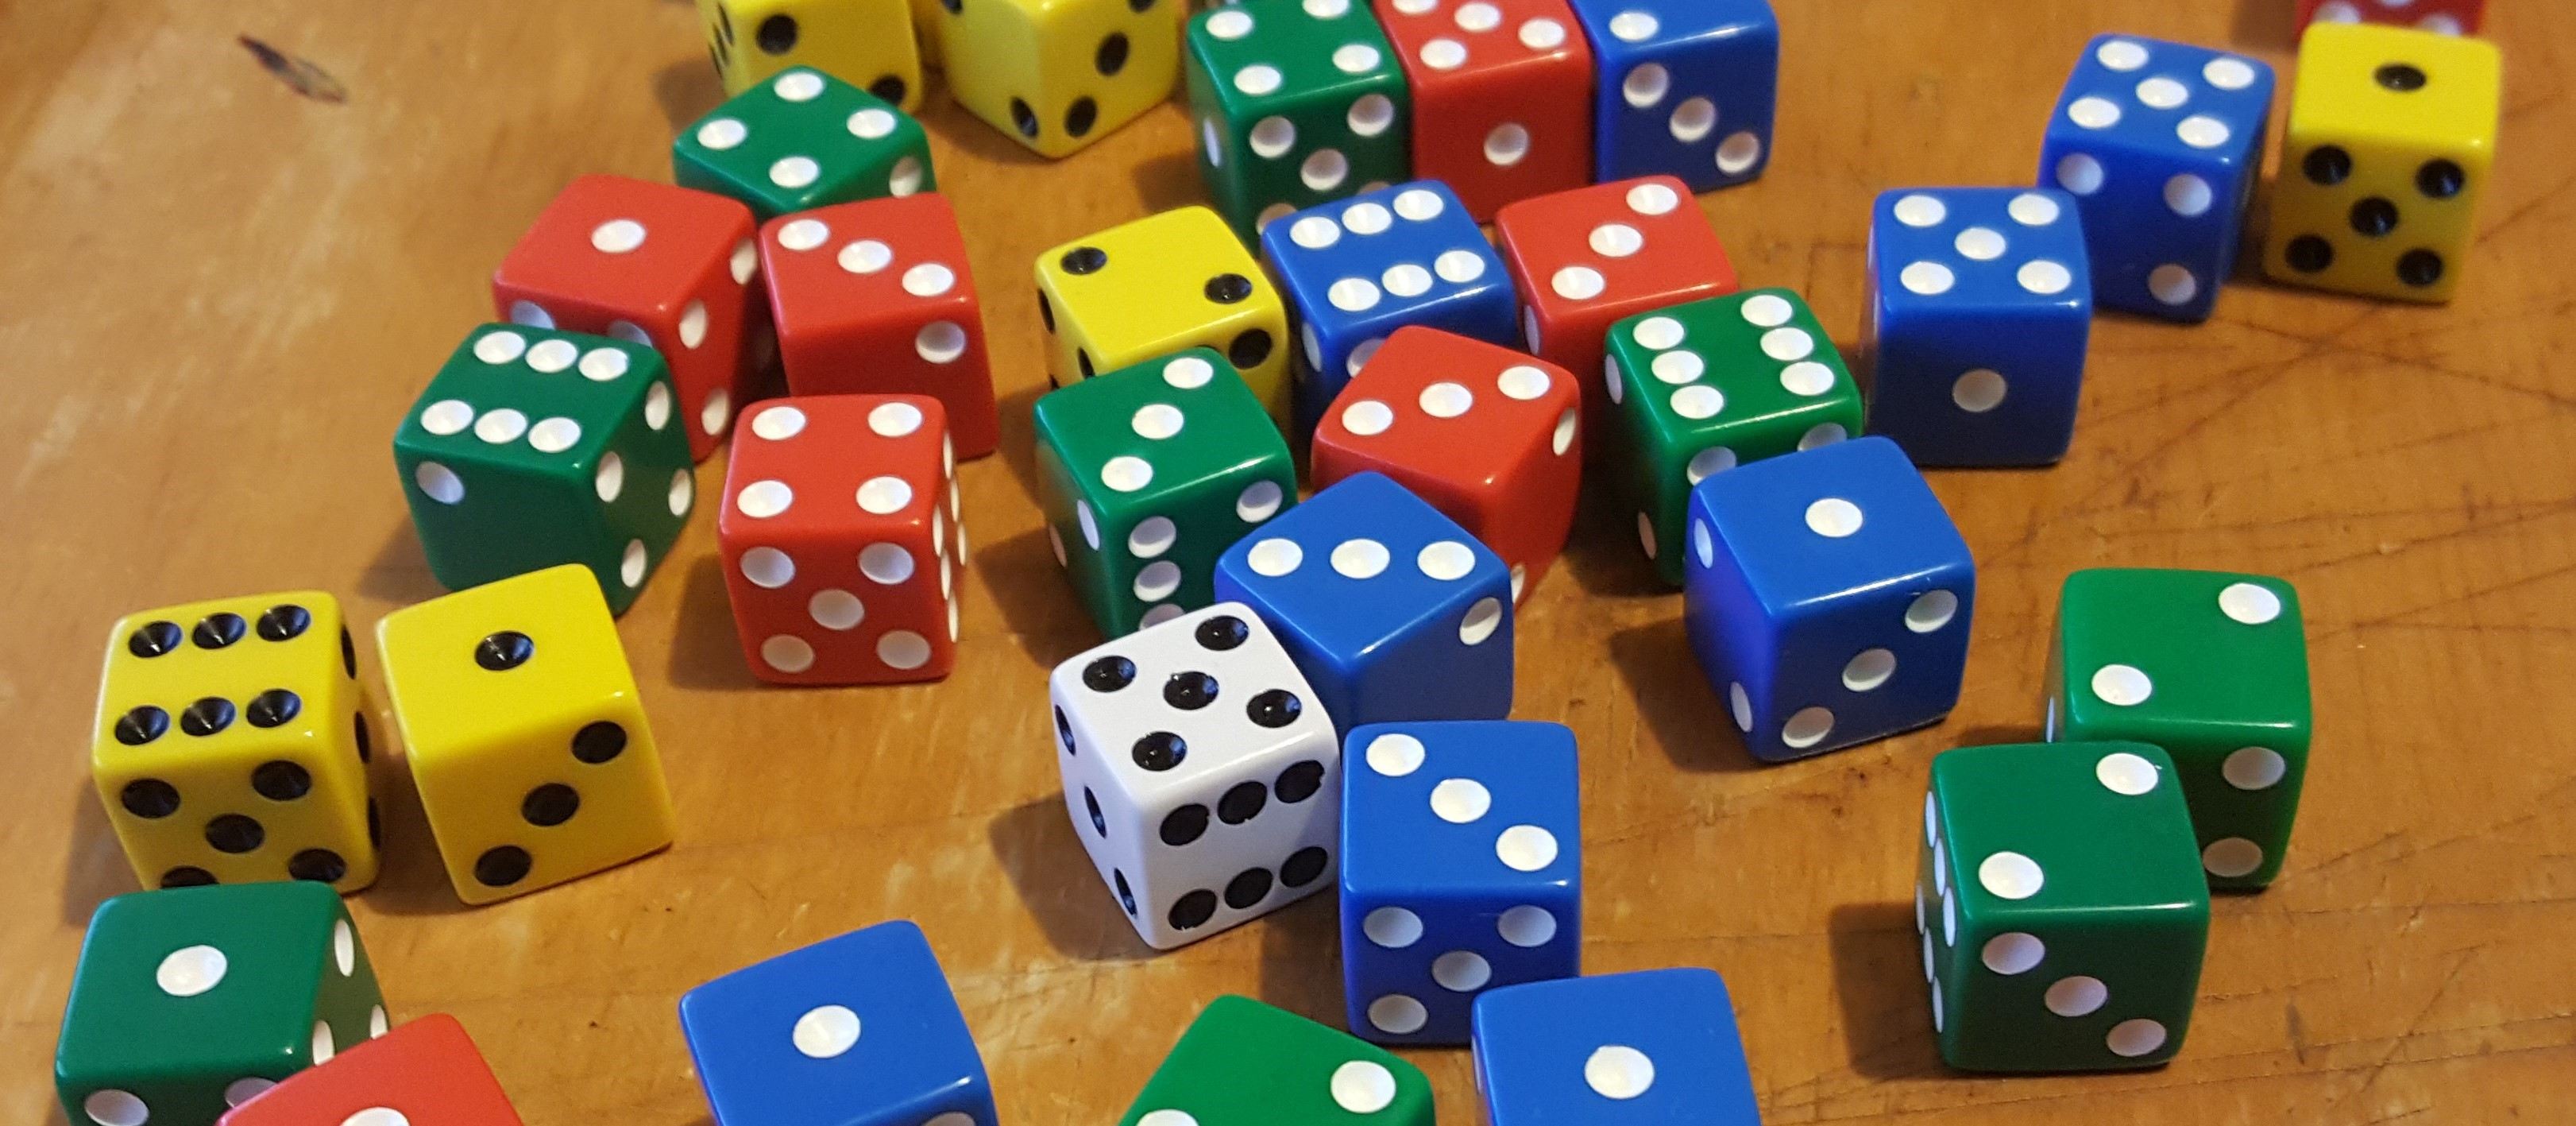
\includegraphics[width=0.4\textwidth]{intro}
	\caption{An assortment of modern plastic dice. Note that not all pip colours are the same across different dice.}
	\label{fig:intro}
\end{figure}

Dice value detection is a valuable tool for the gaming and gambling industries.
Image recognition has often been used in conjunction with other techniques to protect casinos against cheating and to provide a trail of accountability \cite{4129523}\cite{Correia1995}.
Common image processing and feature detection methods can be used to identify the position of dice.
Machine learning algorithms can be used to classify the value of the dice.
With the advent of modern graphics processing units (GPUs), parallel computing has become more widely available and faster than for previous generations of hardware.

The proposed method takes advantage of these advances in consumer-grade technology to detect and classify dice values.

\section{Background}

% Rather than just a summary of prior related research, write a critical review - that is, mention limitations of any prior research/algorithms cited.

Prior research in this field have taken advantage of numerous methods.

\subsection{Prior Research}

The ``SORTE'' system was commissioned by the Portuguese Gaming Inspection Authorities for use in casinos \cite{Correia1995}.
It identified the locations of the pips on all dice and uses spatial locality to assign values to each.
However, this system required specific dice, a birds-eye view of the surface (figure \ref{fig:prior_1a}), and a careful ambient lighting setup.
\begin{figure}
	\centering
	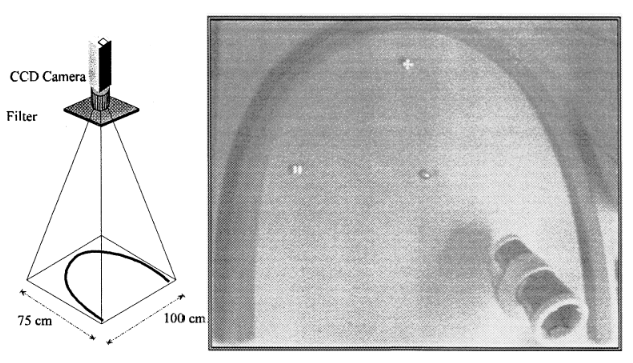
\includegraphics[width=0.4\textwidth]{prior_1a}
	\caption{The apparatus setup including gaming table and camera.}
	\label{fig:prior_1a}
\end{figure}

The system designed by Lapanja, et al., detects dice values for a mechanical gambling machine \cite{Lapanjaa}.
It uses color difference to identify the pips and template matching to classify the value of each die.
This method requires a birds-eye view, a high-contrast background surface, and relies on hard-coded masks for classification.

The system devised by Huang \cite{Huang2008} uses a modified unsupervised gray clustering algorithm. 
However, it requires a birds-eye view, a high-contrast background, and the number of dice to be known in advance.

Finally, the method proposed by Chung \cite{Chung2009} uses the least distance criterion to classify die values.
This method detects the pips and then groups the pips into valid configurations based on the relative distance between each pip.
This method requires a birds-eye view and has only been tested on up to four dice.

Dice detection does not live entirely in the realm of industry and academia.
Amatuers and hobbyists have had success in creating programs that solve this problem \cite{Gideon2018}\cite{Pesce2019}.  

All of these methods rely on detecting the pips and have been constrained by either the camera angle, the number of dice, or the background surface.
The proposed method focuses on detecting the die outline and then classifying the value using a convolutional neural network (CNN).

\section{Method}

The proposed method is arranged in several stages.
Figure \ref{fig:stages} illustrates the process of classifying the dice values from an image. 
\begin{figure}
	\centering
	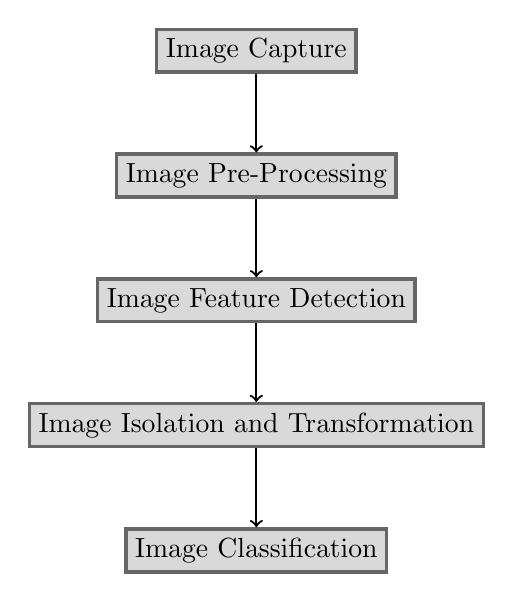
\begin{tikzpicture}[
		rectnode/.style={rectangle, draw=black!60, fill=black!15, very thick, minimum size=5mm},
	]
		
		% nodes
		\node[rectnode] (edge)							{Image Capture};
		\node[rectnode] (contour) 	[below=of edge] 	{Image Pre-Processing};
		\node[rectnode] (size)		[below=of contour] 	{Image Feature Detection};
		\node[rectnode] (shape)		[below=of size]		{Image Isolation and Transformation};
		\node[rectnode] (cnn)		[below=of shape]	{Image Classification};

		% lines
		\draw[thick, ->] (edge.south) -- (contour.north);
		\draw[thick, ->] (contour.south) -- (size.north);
		\draw[thick, ->] (size.south) -- (shape.north);
		\draw[thick, ->] (shape.south) -- (cnn.north);
	\end{tikzpicture}
	\caption{The image processing pipeline.}
	\label{fig:stages}
\end{figure}

\subsection{Image Pre-processing}

The image (figure \ref{fig:original}) is obtained from a source such as a file or video stream.
Pre-processing is performed to remove extraneous information from the image.

% GRAYSCALE
The image is converted to a grayscale color-space.
Equation \ref{eq:rgb2gray} is used to convert an RGB image into grayscale.
It is based on the luminance formula from ``Recommendation BT.601'' \cite{R2011}.
Performing subsequent operations on a grayscale image increases speed at the cost of losing colour information.
\begin{align}
	\textnormal{gray}(R, G, B) &= 0.299 \cdot R + 0.587 \cdot G + 0.114 \cdot B \label{eq:rgb2gray}
\end{align}

% BINARY THRESHOLD
A binary threshold is performed (equation \ref{eq:threshold}).
This reduces the amount of noise present in the image and draws attention to sharp edges (figure \ref{fig:threshold}).
This step is required for the edge detection step.
\begin{align}
	\textnormal{threshold}(x) &= \begin{cases}
		\textnormal{black} & x \leq 160 \\
		\textnormal{white} & \textnormal{otherwise}
	\end{cases} \label{eq:threshold}
\end{align}
\begin{figure}
	\centering
	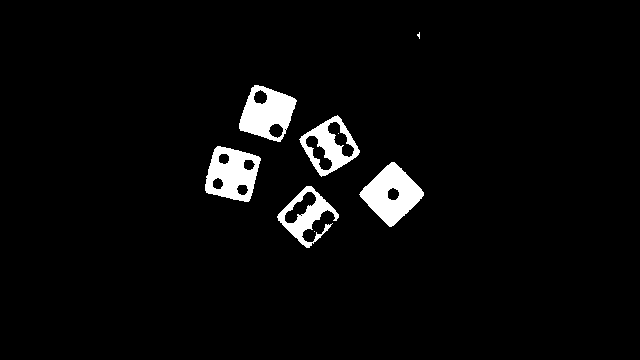
\includegraphics[width=0.4\textwidth]{threshold}
	\caption{The image after thresholding.}
	\label{fig:threshold}
\end{figure}

% GAUSSIAN BLUR
Smoothing is applied to the image to reduce the effect of any remaining noise.
This is typically acheived with a 2-dimensional convolutional filter.
A gaussian kernel of size 5 was chosen for the convolution (equation \ref{eq:kernel}). 
The image (figure \ref{fig:blurred}) is now sufficiently clean of noise and feature detection can take place.
\begin{align}
	K = \{0.0625, 0.25, 0.375, 0.25, 0.0625\}^T \label{eq:kernel}
\end{align}
\begin{figure}
	\centering
	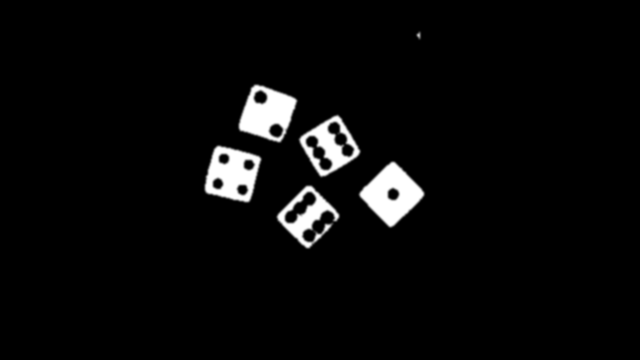
\includegraphics[width=0.4\textwidth]{blur}
	\caption{The image after pre-processing.}
	\label{fig:blurred}
\end{figure}

\subsection{Die Face Detection}

The dice detector stage is broken up into discrete steps.
First the edges are detected using Canny's edge detection algorithm.
Then the edges are joined into contours by Suzuki's contour tracing algorithm.
Finally, the contours are filtered based on their size and shape.
This leaves only the contours that are likely to be die outlines.

\subsubsection{Edge Detection}
% CANNY EDGE DETECTION
The Canny edge detector \cite{Canny1986} is used to find the edges of the dice.
It builds upon the Sobel filter \cite{Sobel2014} which finds extreme vertical and horizontal gradients, $G_x$ and $G_y$, in an image.
The edge gradient, $G$, and angle, $\theta$, for each pixel is then given by equations \ref{eq:gradient} and \ref{eq:angle} respectively.
The edge gradient is always perpendicular to the edge, therefore it is rounded to either horizontal, vertical, or a diagonal.
\begin{align}
	G &= \sqrt{G_x^2 + G_y^2} \label{eq:gradient} \\[1em]
	\theta &= \tan^{-1}\left(\frac{G_y}{G_x}\right) \label{eq:angle}
\end{align}
Every pixel is then checked to ensure it is the local maximum in the direction of the gradient at that point.
This has the effect of making the edges one pixel thin.
Finally, a double threshold is applied to ensure that only the relevant edges are kept.
Any pixels that have a gradient intensity above 320 are considered to be edges.
Any pixels that have a gradient intensity above 110 and are connected to an edge are also considered edges.
A small number of edges that are not related to the dice remain due to variations in lighting and background surface texture (figure \ref{fig:canny}).
\begin{figure}
	\centering
	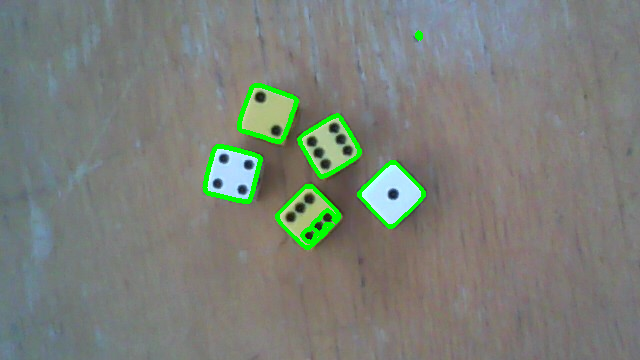
\includegraphics[width=0.4\textwidth]{canny}
	\caption{The original image with the edges highlighted.}
	\label{fig:canny}
\end{figure}

\subsubsection{Contour Tracing}
% SUZUKI CONTOUR TRACING
The Suzuki contour tracing algorithm \cite{Suzuki1985} joins related continuous edges.
It walks over the image and categorises each edge. 
In this way it can create a hierarchy of edge features such as the outer border and hole border.

\subsubsection{Contour Filtering}
% CONTOUR FILTERING
The contours are then kept if they have the following properties:
\begin{itemize}
	\item They have four points (i.e. are quadrilateral).
	\item They have an area greater than 200 pixels square. This removes any small contours that are artifacts of the lighting.
	\item They are square-ish. The shape rejection filter (listing \ref{lst:shape-rejection}) will reject contours that are not square enough.
		The proposed implementation uses an acceptable error of 20\%.
\end{itemize}
\begin{lstlisting}[language=python, caption={The shape rejection filter in Python.}, label={lst:shape-rejection}]
def get_edge_length(p1, p2):
    return np.sqrt(
    	abs(p2[1] - p1[1]) ** 2 +
    	abs(p2[0] - p1[0]) ** 2)

def is_square(points, error):
    [p1, p2, p3, p4] = points
    e1 = get_edge_length(p1, p2)
    e2 = get_edge_length(p2, p3)
    diff = abs(e1 - e2) / max(e1, e2)
    return diff <= error
\end{lstlisting}
After contour filtering is performed only the dice are left (figure \ref{fig:contour}). 
\begin{figure}
	\centering
	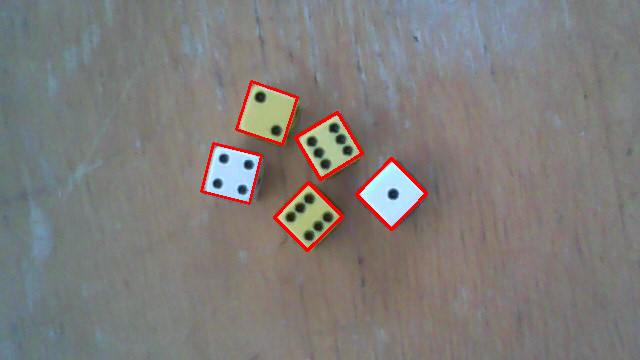
\includegraphics[width=0.4\textwidth]{contours}
	\caption{The original image with the remaining contours highlighted.}
	\label{fig:contour}
\end{figure}

\subsection{Die Face Transformation}

The location and angle of the die face is now known within the original image (figure \ref{fig:canny}).
Each die face must now be transformed before the CNN can be applied.

Each square region must be cropped from the original image and rotated so that it lies flat upon the cartesian axis.
Rotation is performed with an affine rotation transformation.
Each image must be scaled to 64x64 pixels for classification.
The die faces have been isolated (figure \ref{fig:faces}) and can now be passed to the CNN for classification.
\begin{figure}
	\centering
	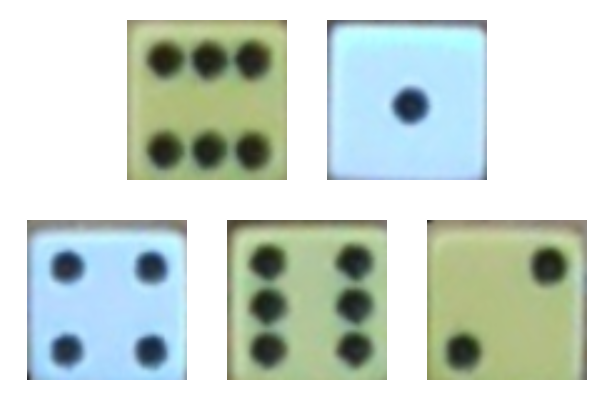
\includegraphics[width=0.3\textwidth]{faces}
	\caption{The die faces after transformation.}
	\label{fig:faces}
\end{figure}

\subsection{Machine Learning}

Machine learning algorithms are often used to solve problems that would be difficult to solve using traditional computing methods \cite{Goodfellow2016}.
A CNN is a class of deep neural networks that has many applications in computer vision, speech recognition, and many other fields \cite{Pena2014}\cite{Madabhushi2016}\cite{Lawrence1997}\cite{Kalchbrenner2014}.
A deep neural network is designed with many layers where the information will pass through.
A model will then be trained on a large dataset with known parameters.
This model can then be used to classify images that it hasn't seen before.

The proposed CNN has 4 layers and uses categorical cross-entropy as its loss function. 
This allows the model to produce probabilities for all six values while being aware that only one is correct.
The model was trained on 1200 images of white and yellow dice that were manually captured and classified.
Each image is grayscale and 64x64 pixels in size.

\subsection{Die Classification}

The CNN determines the probability that the isolated die face has a specific number value.
The largest of these values is selected and the original image is annotated with the most likely number for each dice (figure \ref{fig:annotated}).
\begin{figure}
	\centering
	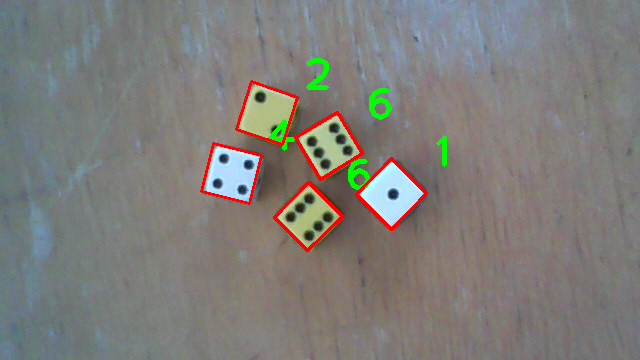
\includegraphics[width=0.4\textwidth]{annotated}
	\caption{The final image with annotations.}
	\label{fig:annotated}
\end{figure}

\section{Results}

A laptop with the following hardware specifications was used for testing:
\begin{itemize}
	\item $\SI{2.4}{\giga\hertz}$ Intel Core i5 processor,
	\item $\SI{8}{\giga\byte}$ of memory.
\end{itemize}

A proof-of-concept program was written.
The following software was used to run the program:
\begin{itemize}
	\item Python $3.8.1$,
	\item OpenCV $4.2.0$,
	\item Tensorflow $2.2.0$,
	\item Windows 10 (64-bit).
\end{itemize}

A Logitech C170 webcam with a resolution of 640x360 pixels was used to capture images and videos.
A wooden desk was used as hard surface where the dice could be rolled.
A desk lamp was used to improve the ambient lighting on the desk. 

The webcam was setup approximately $\SI{27}{\centi\metre}$ above the surface looking directly down (figure \ref{fig:test}). 
Two white dice (black pips) and two yellow dice (black pips) were rolled 50 times.
The webcam was paused while the results were recorded in a spreadsheet.
\begin{figure}
	\centering
	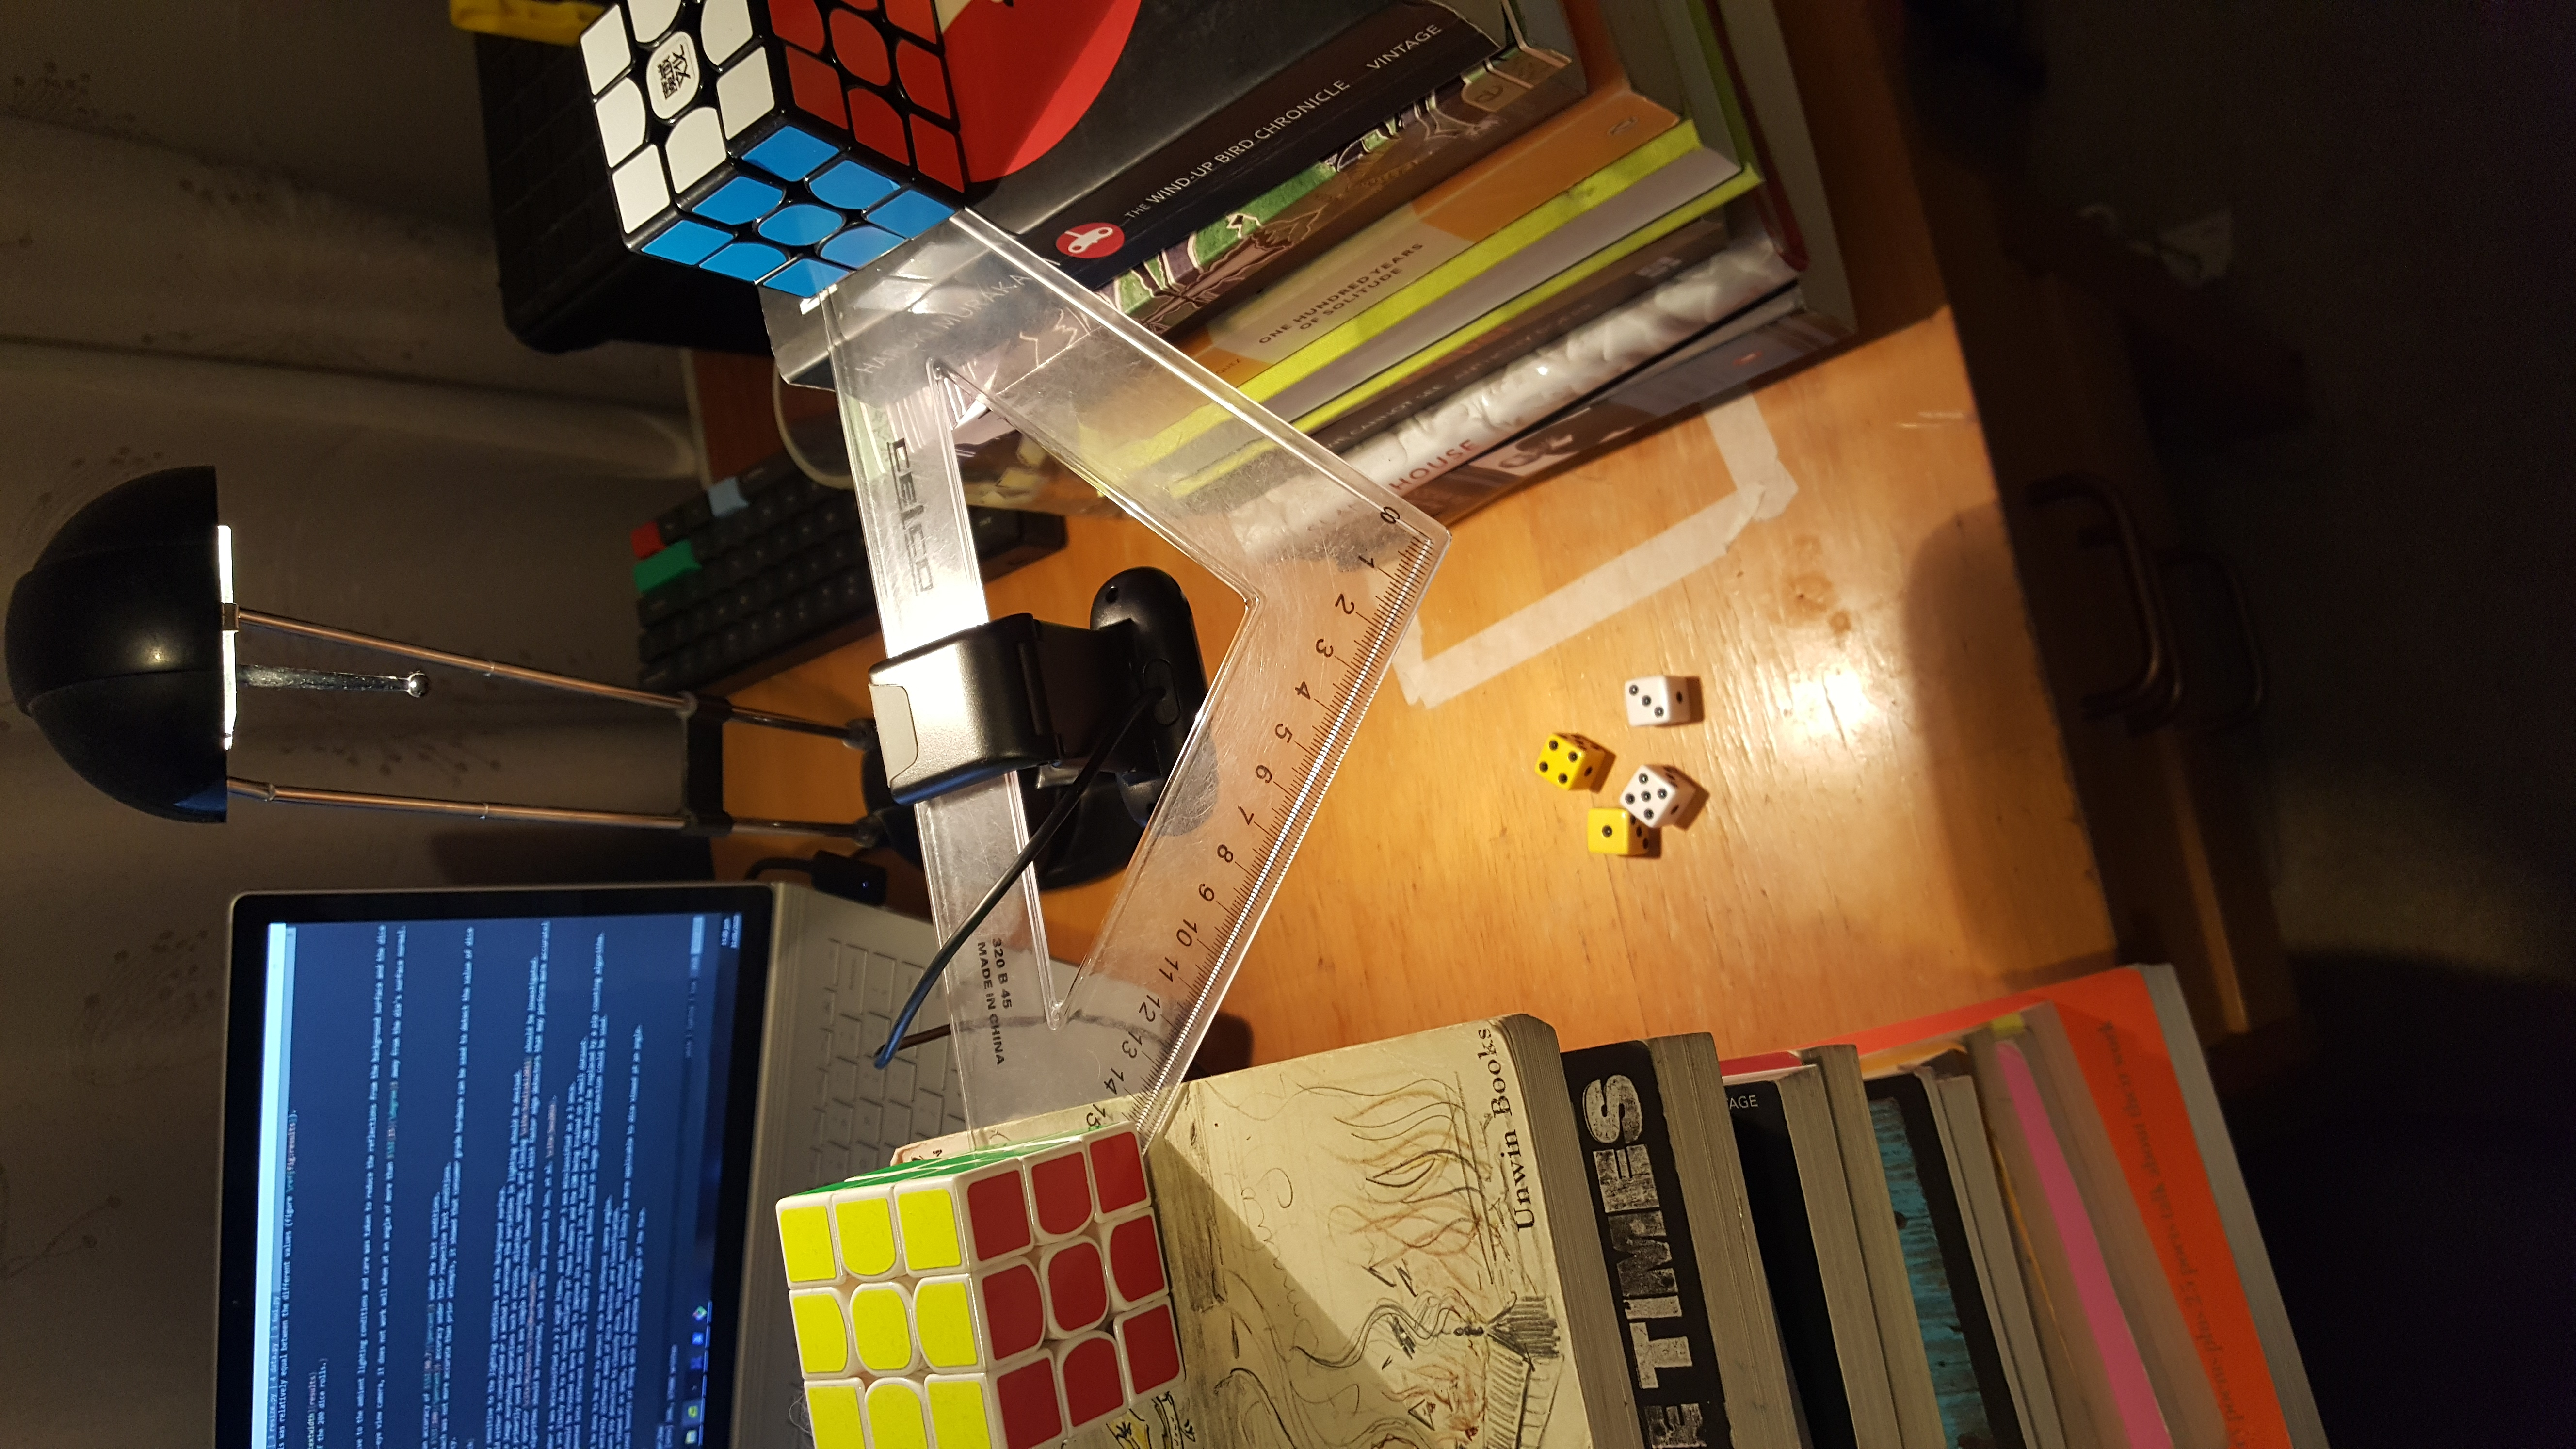
\includegraphics[width=0.7\textwidth, angle=270, origin=c]{test}
	\caption{The test apparatus.}
	\label{fig:test}
\end{figure}

Over the 200 rolls, $\SI{95.0}{\percent}$ of the dice were detected, and $\SI{95.5}{\percent}$ of these were correctly classified.
This yields an overall accuracy of $\SI{90.7}{\percent}$.
The distribution of the dice rolls was relatively equal between the different values (figure \ref{fig:results}).
\begin{figure}
	\centering
	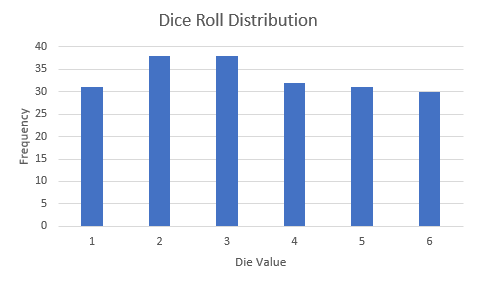
\includegraphics[width=0.5\textwidth]{results}
	\caption{The distribution of the 200 dice rolls.}
	\label{fig:results}
\end{figure}

The proposed method is sensitive to the ambient lighting conditions and care was taken to reduce the reflections from the background surface and the dice themselves.
This method also uses a birds-eye view camera, it does not work well when at an angle of more than $\SI{15}{\degree}$ away from the die's surface normal.

\section{Conclusion}

The proposed method yields an accuracy of $\SI{90.7}{\percent}$ under the test conditions.
All prior research showed a $\SI{100}{\percent}$ accuracy under their respective test conditions.
Although the proposed approach was not more accurate than prior attempts, it showed that consumer grade hardware can be used to detect the value of dice with high levels of accuracy.

\subsection{Future Research}

The dice detector is very sensitive to the lighting conditions and the background surface.
In the future, this should either be constrained or a method to overcome the variations in lighting should be devised.
More experimentation into image morphology operations such as erosion, dilation, opening, and closing \cite{Szeliski2011} should be investigated.
Canny edge detection was primarily used because it was simple to understand, however there do exist faster edge detectors that may perform more accurately, such as the declivity operator \cite{Mich1995}\cite{Bhardwaj2012}.
Faster contour tracing algorithms should be researched, such as the one proposed by Seo, et al. \cite{Seo2016}.

During testing, the number 4 was misclassified as a 2 eight times, and the number 5 was misclassified as a 3 once.
The misclassifications are likely due to the visual similarity of these numbers and the CNN being trained on a small dataset. 
Either the CNN model should be trained on more images to improve its accuracy in the future or the CNN should be replaced by a pip counting algorithm.
Once the image is segmented into different die faces, a simple pip counting method based on image feature detection could be used.

Further research must be done to be able to detect dice from different camera angles.
This may involve an entirely different model of dice detection and classification.
All prior research uses pip detection to classify dice, this method would likely be more applicable to dice viewed at an angle.
This is because when viewed at an angle, each pip becomes elliptical.
This has the additional benefit of being able to determine the angle of the face.

\printbibliography

\end{document}
